%% http://latex.informatik.uni-halle.de/latex-online/latex.php

\documentclass[12pt,preprint]{aastex}



%%% PACKAGES %%%%%%%%%%%%%%%%%%%%%%%%%%%%%%%%%%%%%%%%%%%%%%%%%%%%%%%%%%%%%%%%%%%

\usepackage{amsmath}
\usepackage{xspace}   % fixes spaces after custom commands
\usepackage{float}    % exact placement of figures (using \begin{figure}[H])
\usepackage{color}  % well... color...
\usepackage{subfigure}

\usepackage{longtable}   % those two to generate the 2 ol table
\usepackage{multicol}

%%% DEFINITIONS %%%%%%%%%%%%%%%%%%%%%%%%%%%%%%%%%%%%%%%%%%%%%%%%%%%%%%%%%%%%%%%%

\def\half{{\textstyle\frac12}}
% makes it easier to have consistent writing, and easy change if needed
\newcommand{\spl}{SpaghettiLens\xspace}
\newcommand{\sw}{SpaceWarps\xspace}

% shortcut for einstein radius (Text Greek Full Math)
\newcommand{\ER}{Einstein radius\xspace} % text
\newcommand{\ERg}[1][]{$\Theta_\text{E#1}$\xspace} % er in textmode with greek
\newcommand{\ERf}[1][]{Einstein radius $\Theta_\text{E#1}$\xspace} % full output
\newcommand{\ERm}[1][]{\Theta_\text{E#1}} % mathmode with greek symbol

%shortcuts for kappa
\newcommand{\kenc}[1][r]{$\kappa_\text{encl}(#1)$\xspace}
\newcommand{\kap}[1][r]{$\kappa(#1)$\xspace}

% shorcuts for refs (use capital for beginning of sentence)
% first 3 are for the real layz people..
\newcommand{\fref}[1]{\ref{fig:#1}}
\newcommand{\sref}[1]{\ref{sec:#1}}
\newcommand{\tref}[1]{\ref{tab:#1}}
\newcommand{\figref}[1]{Figure~\ref{fig:#1}}
\newcommand{\secref}[1]{Section~\ref{sec:#1}}
\newcommand{\tabref}[1]{Table~\ref{tab:#1}}
\newcommand{\Figref}[1]{Figure~\ref{fig:#1}}
\newcommand{\Secref}[1]{Section~\ref{sec:#1}}
\newcommand{\Tabref}[1]{Table~\ref{tab:#1}}

% shortcut for ASW000xxxx
\newcommand{\asw}[1]{ASW000#1\xspace}

%shorcut for model (maybe link later to appendix)
% use \model{4356} for with text and
% \model[]{3456} for only number
\newcommand{\model}[2][Model~]{#1#2\xspace}


%degrees
\newcommand{\dgr}{^{\circ}}


% todo annotations on side in red. easy to search for at the end
\newcommand{\todo}[2][red]{%\marginpar{\raggedright\scriptsize\sffamily\textcolor{red}{#1}}}
%{\marginpar{\raggedright\sffamily\textcolor{red}\footnotesize
%\setstretch{1.025}%
%#1}}}
\textcolor{#1}{\textbullet}%
\marginpar{\colorbox{#1}{\parbox{\marginparwidth}{%
\setstretch{0.4}\sffamily\textcolor{black}{\scriptsize{#2}}}}}}

\newcommand{\needfig}[1][]{%
\colorbox{yellow}{\parbox{0.5\textwidth}{%
\vspace{0.5cm}\setstretch{0.5}\textcolor{black}{\scriptsize{fig #1}}\vspace{0.5cm}}}%
\marginpar{\colorbox{yellow}{\parbox{\marginparwidth}{%
\setstretch{0.4}\sffamily\textcolor{black}{\scriptsize{fig}}}}}}

\setlength{\marginparsep}{0mm}
\setlength{\marginparwidth}{2.2cm}

% quick todo annotations
\newcommand{\needcite}[1][]{\todo[green]{cit #1}}
\newcommand{\needref}[1][]{\todo[cyan]{ref #1}}
\newcommand{\needchk}[1][]{\todo[red]{chk #1}}

\newcommand{\hr}{\vspace{5mm}\noindent\rule{0.8\textwidth}{0.4pt}\vspace{5mm}}




%%% DOCUMENT %%%%%%%%%%%%%%%%%%%%%%%%%%%%%%%%%%%%%%%%%%%%%%%%%%%%%%%%%%%%%%%%%%%
\begin{document}
\section{\Large Gravitational Lensing formalism }

In general relativity, a point mass deflects a light ray with impact parameter \(b\) by an angle \[\hat{\alpha} = \frac{4GM}{c^2b}\] where G is the Gravitational constant, M the mass of the deflecting object  and c the speed of light. A naive application of Newtonian gravity can yield exactly half this value, where the light ray is assumed as a massed particle and scattered by the gravitational potential well.
In situations where General Relativity can be approximated by linearized gravity, the deflection due to a spatially extended mass can be written simply as a vector sum over point masses.  In the continuum limit, this becomes an integral over the density \(\rho \), and if the deflection is small we can approximate the gravitational potential along the deflected trajectory by the potential along the undeflected trajectory, as in the Born approximation in Quantum Mechanics.  The deflection is then
\[\vec{\hat{\alpha}}(\vec{\xi})=\frac{4 G}{c^2} \int d^2\xi^{\prime} \int dz \rho(\vec{\xi}^{\prime},z)  \frac{\vec{b}}{|\vec{b}|^2}, ~ \vec{b} \equiv \vec{\xi}  - \xi^{\prime} \]
where \(z\) is the line-of-sight coordinate, and \( \vec{b} \) is the vector impact parameter of the actual ray path from the infinitesimal mass \[  d^2\xi^{\prime}  dz\rho(\vec{\xi}^{\prime},z) \] located at the coordinates \[(\vec{\xi}^{\prime}, z)\]
% cite >{{ cite journal | last = Bartelmann| first = M. | coauthors = Schneider, P. | year = 2001 | month = January | title=Weak Gravitational Lensing| journal = Physics Reports D | volume=340 | issue = 4�5 |pages = 291�472 | bibcode = 2001PhR...340..291B | doi = 10.1016/S0370-1573(00)00082-X|arxiv = astro-ph/9912508 }}

\textbf{Thin lens approximation}

In the limit of a "thin lens", where the distances between the source, lens, and observer are much larger than the size of the lens (this is almost always true for astronomical objects), we can define the projected mass density

\[\Sigma(\vec{\xi})=\int \rho(\vec{\xi},z) dz \]

where \(\vec{\xi}\) is a vector in the plane of the sky.  The deflection angle is then

\[\vec{\hat{\alpha}}= 
\frac{4 G}{c^2} \int \frac{(\vec{\xi}-\vec{\xi}^{\prime})\Sigma(\vec{\xi}^{\prime})}{|\vec{\xi}-\vec{\xi}^{\prime}|^2}d^2 \xi^{\prime 2}\]


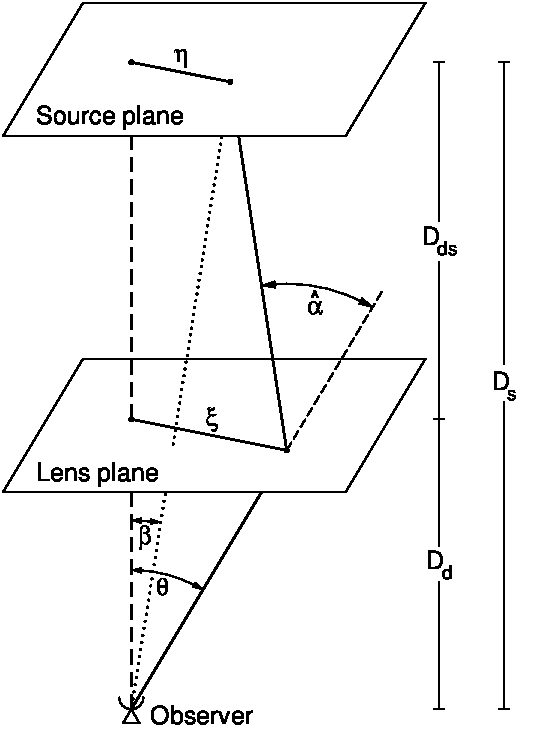
\includegraphics[scale=0.5]{../fig/lens-sketch.png}
\caption{\\fig. Sketch of a typical gravitational lens system \footnotesize [Bartelmann, Schneider 2001] }

As shown in the diagram, the difference between the unlensed angular position \(\vec{\beta}\) and the observed position \(\vec{\theta}\) is this deflection angle, reduced by a ratio of distances, described as the lens equation

\[\vec{\beta}=\vec{\theta}-\vec{\alpha}(\vec{\theta}) = \vec{\theta} - \frac{D_{ds}}{D_s} \vec{\hat{\alpha}}(\vec{D_d\theta})\]

where \(D_{ds}\) is the distance from the lens to the source \(D_s\) is the distance from the observer to the source, and \(D_d\) is the distance from the observer to the lens.  For extragalactic lenses, these must be angular diameter distances.

In strong gravitational lensing, this equation can have multiple solutions, because a single source at \(\vec{\beta}\) can be lensed into multiple images.

\pagebreak
\textbf{Convergence and deflection potential}

It is convenient to define the "convergence"

\[
\kappa(\vec{\theta}) = \frac{\Sigma(D_d\vec{\theta})}{\Sigma_{cr}}
\]

and the "critical surface density" (not to be confused with the Critical density (cosmology) of the universe)

\[
\Sigma_{cr} = \frac{c^2 D_s}{4\pi G D_{ds}D_d}
\]

The reduced deflection angle \(\vec{\alpha}(\vec{\theta})\) can now be written as

\[
\vec{\alpha}(\vec{\theta}) = \frac{1}{\pi}\int d^2 \theta^{\prime} \frac{(\vec{\theta}-\vec{\theta}^{\prime})\kappa(\vec{\theta}^{\prime})}{|\vec{\theta}-\vec{\theta}^{\prime}|^2}
\]

We can also define the "`deflection potential"'

\[
\psi(\vec{\theta}) = \frac{1}{\pi}\int d^2 \theta^{\prime} \kappa(\vec{\theta}^{\prime}) \ln |\vec{\theta}-\vec{\theta}^{\prime}|
\]

such that the scaled deflection angle is just the gradient of the potential and the convergence is half the Laplacian of the potential:

\[
\vec{\alpha}(\vec{\theta}) = \vec{\nabla} \psi(\vec{\theta})
\]

\[
\kappa(\vec{\theta}) = \frac{1}{2} \nabla^2 \psi(\vec{\theta})
\]

The deflection potential can also be written as a scaled projection of the Newtonian gravitational potential \(\Phi\) of the lens

%%% {{ cite journal | last = Narayan| first = R. | coauthors = Bartelmann, M. | year = 1996 | month = June | title=Lectures on Gravitational Lensing| journal = Eprint arXiv:astro-ph/9606001 | bibcode =1996astro.ph..6001N |arxiv = astro-ph/9606001 | last2 = Bartelmann | pages = 6001 }}


\[
\psi(\vec{\theta}) = \frac{2 D_{ds}}{D_d D_s c^2} \int \Phi(D_d\vec{\theta},z) dz
\]

\pagebreak
\textbf{Lensing Jacobian}

The Jacobian matrix and determinant between the unlensed and lensed coordinate systems is

\[A_{ij}=\frac{\partial \beta_i}{\partial \theta_j}=\delta_{ij} - \frac{\partial \alpha_i}{\partial \theta_j}
= \delta_{ij} - \frac{\partial^2 \psi}{\partial \theta_i \partial \theta_j}\]

where \(\delta_{ij}\) is the Kronecker delta.  Because the matrix of second derivatives must be symmetric, the Jacobian can be decomposed into a diagonal term involving the convergence and a matrix trace-free term involving the "shear" \(\gamma \) 

\[A=(1-\kappa)\left[\begin{array}{ c c } 1 & 0 \\ 0 & 1 \end{array}\right]-\gamma\left[\begin{array}{ c c } \cos 2\phi & \sin 2\phi \\ \sin 2\phi & -\cos 2\phi \end{array}\right]\]

where \(\phi\) is the angle between \(\vec{\alpha}\) and the x-axis.  The term involving the convergence magnifies the image by increasing its size while conserving surface brightness.  The term involving the shear stretches the image tangentially around the lens, as discussed in Weak lensing observables.

The shear defined here is 'not' equivalent to the shear mapping traditionally defined in mathematics, though both stretch an image non-uniformly.



\textbf{Fermat Surface}

There is an alternative way of deriving the lens equation, starting from the photon arrival time (Fermat surface) 	

\[
t =  \int_{0}^{z_s}   { n dz \over c \cos \alpha(z) } 
\] 

where \( dz/c \) is the time to travel an infinitesimal line element along the source-observer straight line in vacuum, which is 
then corrected by the factor 

\[
1/\cos(\alpha(z))  \approx 1 + {\alpha(z)^2 \over 2}
\]

to get the line element along the bended path \[ dl = {dz \over c \cos \alpha(z) } \]  with a varying small pitch angle \( \alpha(z)\), and the refraction index  
\(n \) for the "aether", i.e., the gravitational field.  The last can be obtained from the fact that a photon travels on a null geodesic of a weakly perturbed static Minkowski universe 

\[
ds^2 = 0  = c^2 dt^2 \left(1 + {2 \Phi \over c^2} \right) -  \left(1 + {2 \Phi \over c^2} \right)^{-1} dl^2
\]
 
where  the uneven gravitational potential \[ \Phi \ll c^2 \] drives a changing the speed of light 

\[
c' = {dl/dt} = \left(1 + {2 \Phi \over c^2} \right)  c
\]

So the refraction index
 
\[
 n \equiv {c \over c'} \approx  \left(1 -  {2 \Phi \over c^2} \right) 
\]

The refraction index greater than unity because of the negative gravitational potential \( \Phi \).

Put these together and keep the leading terms we have the time arrival surface 

\[ 
t \approx \int_0^{z_s} {dz \over c}  +  \int_0^{z_s} {dz \over c} {\alpha(z)^2 \over 2} -  \int_0^{z_s} {dz \over c} {2 \Phi \over c^2} 
\]

The first term is the straight path travel time, the second term is the extra geometric path, and the third is the gravitational delay. 
Make the triangle approximation that \[ \alpha(z) = \theta - \beta \] for the path between the observer and the lens, 
and \[ \alpha(z) \approx (\theta - \beta) {D_d \over D_{ds}} \] for the path between the lens and the source.  
The geometric delay term becomes

\[
    {D_d \over c}   { (\vec{\theta} - \vec{\beta})^2 \over 2} 
+ {D_{ds} \over c}  { \left[ (\vec{\theta} - \vec{\beta} )  {D_d \over D_{ds}} \right]^2 \over 2}
= {D_d D_s \over D_{ds} }    { ( \vec{\theta} - \vec{\beta} )^2 \over 2}
\]

So the Fermat surface becomes 

\[
 t = constant + {D_d D_s \over D_{ds} c} \tau, ~ \tau \equiv \left[  { (\vec{\theta}-\vec{\beta})^2 \over 2} -  \psi \right] 
\]

where \( \tau \) is so-called dimensionless time delay, and the 2D lensing potential  

\[
\psi(\vec{\theta}) = \frac{2 D_{ds}}{D_d D_s c^2} \int \Phi(D_d\vec{\theta},z) dz
\]
 
The images lie at the extrema of this surface, so the variation of \(t \) with \(\vec{\theta} \) is zero, 

\[
0 = \nabla_{\vec{\theta}} \tau  =  \vec{\theta} - \vec{\beta}  - \nabla_{\vec{\theta}} \psi(\vec{\theta}) 
\]

which is the lens equation.  Take the Poisson's equation for 3D potential 
\[
\Phi(\vec{\xi})  = - \int  \frac{d^3\xi^{\prime} \rho(\vec{\xi}^{\prime})}{|\vec{\xi}-\vec{\xi}^{\prime}|} 
\]

and we find the 2D lensing potential 

\[\psi(\vec{\theta})   = - \frac{2 G D_{ds}}{D_d D_s c^2}   \int dz  \int  \frac{d^3\xi^{\prime} \rho(\vec{\xi}^{\prime})}{|\vec{\xi}-\vec{\xi}^{\prime}|}
 =  -  \sum_i \frac{2 G M_i D_{is} }{D_s D_i c^2}   \left[  \sinh^{-1}  { |z -D_i| \over D_i |\vec{\theta}-\vec{\theta}_i |  }  \right ] |_{D_i}^{D_s}  + |_{D_i}^{0}
\]

Here we assumed the lens is a collection of point masses \( M_i \) at angular coordinates \( \vec{\theta}_i \) and distances \[ z=D_i\]  
Use \[ \sinh^{-1} 1/x = \ln(1/x + \sqrt{1/x^2+1}) \approx -\ln(x/2) \] for very small \(x \) we find 

\[
\psi(\vec{\theta})   \approx   \sum_i  \frac{2 GM_i D_{is} }{D_s D_i c^2}   \left[   \ln\left( { |\vec{\theta}-\vec{\theta}_i |^2 \over 4}  { D_i \over D_{is} } \right)     \right]
\]

One can  compute the ''convergence'' by applying the 2D Laplacian of the 2D lensing potential 

\[
\kappa(\vec{\theta}) = \frac{1}{2} \nabla_{\vec{\theta}}^2 \psi(\vec{\theta}) =  \frac{4\pi G D_{ds}D_d} {c^2 D_s} \int dz \rho( D_d \vec{\theta},z) 
== {\Sigma \over \Sigma_{cr} } == \sum_i { 4\pi G M_i D_{is} \over c^2 D_i D_s}  \delta(\vec{\theta}-\vec{\theta}_i)
\]

in agreement with earlier definition \[ \kappa(\vec{\theta}) =  {\Sigma \over \Sigma_{cr} }\] as the ratio of projected density with the critical density.  
Here we used \[ \nabla^2 1/r = - 4 \pi \delta(r) \] and \[  \nabla_{\vec{\theta}} = D_d \nabla \]

We can also confirm the previously defined reduced deflection angle 

\[
\vec{\theta} -\vec{\beta}   =  \nabla_{\vec{\theta}} \psi(\vec{\theta}) =  \sum_i   {  \theta_{Ei}^2  \over |\vec{\theta}-\vec{\theta}_i |} , ~ 
\pi \theta_{Ei}^2 \equiv  {4 \pi GM_i D_{is}  \over c^2 D_s  D_i } 
\]

where \( \theta_{Ei} \) is the so-called Einstein angular radius of a point lens \(Mi \).   For a single point lens at the origin we recover the standard result 
that there will be two images at the two solutions of the essentially quadratic equation 

\[ \vec{\theta} -\vec{\beta}   =   {\theta_{E}^2  \over |\vec{\theta} |} \] 

The amplification matrix can be obtained by double derivatives of the dimensionless time delay 

\[
A_{ij} = {\partial \beta_j \over \partial \theta_i} = {\partial \tau \over \partial \theta_i \partial \theta_j } = \delta_{ij} -  {\partial \psi \over \partial \theta_i \partial \theta_j } 
= \left[\begin{array}{ c c } 1-\kappa -\gamma_1 & \gamma_2 \\ \gamma_2 & 1-\kappa +\gamma_1 \end{array}\right]  \]

where we have define the derivatives 

\[ \kappa = {\partial \psi \over 2 \partial \theta_1 \partial \theta_1 } +  {\partial \psi \over 2\partial \theta_2 \partial \theta_2 } , 
~ \gamma_1 \equiv  {\partial \psi \over 2 \partial \theta_1 \partial \theta_1 } -  {\partial \psi \over 2\partial \theta_2 \partial \theta_2 } ,   
~ \gamma_2 \equiv  {\partial \psi \over \partial \theta_1 \partial \theta_2 }    \]

which takes the meaning of convergence and shear.   The amplification is the inverse of the Jacobian 

\[   A = 1/det(A_{ij}) = {1 \over (1-\kappa)^2 -\gamma_1^2 -\gamma_2^2}  \]

where a positive A means either a maxima or a minima, and a negative A means a saddle point in the arrival surface.

For a single point lens, one can show (albeit a lengthy calculation) that 

\[ \kappa =0, ~ \gamma = \sqrt{\gamma_1^2 + \gamma_2^2} = {\theta_E^2 \over |\theta|^2}, ~ \theta_E^2= {4GM D_{ds} \over c^2 D_dD_s}
\]

So the amplification of a point lens is given by 

\[
A = \left( 1 - {\theta_E^4 \over \theta^4} \right)^{-1}
\]

Note A diverges for images at the Einstein radius \( \theta_E \).

In cases there are multiple point lenses plus a smooth background of (dark) particles of surface density \(\Sigma_{\rm cr} \kappa_{\rm smooth}\), the time arrival surface is 

\[
\psi(\vec{\theta})   \approx   {1 \over 2} \kappa_{\rm smooth} |\theta|^2 +  \sum_i  \theta_E^2  \left[   \ln\left( { |\vec{\theta}-\vec{\theta}_i |^2 \over 4}  { D_d \over D_{ds} } \right)     \right] 
\]

To compute the amplification, e.g., at the origin (0,0), due to identical point masses distributed at \((\theta_{xi},\theta_{yi} ) \) 
we have to add up the total shear, and include a convergence of the smooth background, 
\[
A = \left[ (1 - \kappa_{\rm smooth})^2  
                  - \left( \sum_i {  (\theta_{xi}^2 - \theta_{yi}^2 ) \theta_E^2 \over (\theta_{xi}^2 + \theta_{yi}^2)^2 }\right) ^2  
                  - \left( \sum_i {  (2 \theta_{xi} \theta_{yi}) \theta_E^2 \over (\theta_{xi}^2 + \theta_{yi}^2)^2 }  \right)^2   \right] ^{-1}
\]

This generally creates a network of critical curves, lines connecting image points of infinite amplification.

\end{document}

